%%%%%%%%%%%%%%%%%%%%%%%%%%%%%%%%%%%%%%%%%
% Academic Title Page
% LaTeX Template
% Version 2.0 (17/7/17)
%
% This template was downloaded from:
% http://www.LaTeXTemplates.com
%
% Original author:
% WikiBooks (LaTeX - Title Creation) with modifications by:
% Vel (vel@latextemplates.com)
%
% License:
% CC BY-NC-SA 3.0 (http://creativecommons.org/licenses/by-nc-sa/3.0/)
% 
% Instructions for using this template:
% This title page is capable of being compiled as is. This is not useful for 
% including it in another document. To do this, you have two options: 
%
% 1) Copy/paste everything between \begin{document} and \end{document} 
% starting at \begin{titlepage} and paste this into another LaTeX file where you 
% want your title page.
% OR
% 2) Remove everything outside the \begin{titlepage} and \end{titlepage}, rename
% this file and move it to the same directory as the LaTeX file you wish to add it to. 
% Then add \input{./<new filename>.tex} to your LaTeX file where you want your
% title page.
%
%%%%%%%%%%%%%%%%%%%%%%%%%%%%%%%%%%%%%%%%%

%----------------------------------------------------------------------------------------
%	PACKAGES AND OTHER DOCUMENT CONFIGURATIONS
%----------------------------------------------------------------------------------------

\documentclass[11pt]{article}

\usepackage[utf8]{inputenc} % Required for inputting international characters
\usepackage[T1]{fontenc} % Output font encoding for international characters
\usepackage{graphicx}
\usepackage{mathpazo} % Palatino font
\usepackage[legalpaper,margin=0.9in] {geometry}
\usepackage{fancyhdr}
\usepackage{float}

\setcounter{tocdepth}{4}
\setcounter{secnumdepth}{4}


\pagestyle{fancy}
\fancyhf{}
\lhead{\textsc{University of Regina}}
\rhead{\textsc{Software Systems Engineering}}
\cfoot{\thepage}

\begin{document}

%----------------------------------------------------------------------------------------
%	TITLE PAGE
%----------------------------------------------------------------------------------------

\begin{titlepage} % Suppresses displaying the page number on the title page and the subsequent page counts as page 1
	\newcommand{\HRule}{\rule{\linewidth}{0.5mm}} % Defines a new command for horizontal lines, change thickness here
	
	\center % Centre everything on the page
	
	%------------------------------------------------
	%	Headings
	%------------------------------------------------
	
	\textsc{\Huge University of Regina}\\[1.5cm] % Main heading such as the name of your university/college

	\textsc{\Large ENSE 477: Software Capstone Project}\\[0.5cm]
	
	\textsc{\Large Software Systems Engineering}\\[0.5cm] % Major heading such as course name
	
	
	
	
	%------------------------------------------------
	%	Title
	%------------------------------------------------
	
	\HRule\\[0.4cm]
	
	{\Huge\bfseries Workshop Enterprise Resource Planning Suite User Manual}\\[0.4cm] % Title of your document
	
	\HRule\\[1.5cm]
	
	%------------------------------------------------
	%	Author(s)
	%------------------------------------------------
	
	\begin{minipage}[t]{0.4\textwidth}
		\begin{flushleft}
			\large
			\textsc{Authors}\\
			Jonathan Wells\\
			\textsc{200328640}\\ % Your name
			\large
			Konstantin Kharitonov\\
			\textsc{200354502} % Supervisor's name
		\end{flushleft}
		
	\end{minipage}
	~
	\begin{minipage}[t]{0.4\textwidth}
		\begin{flushright}
			\large
			\textsc{Supervisor}\\ % Supervisor's name
			Karim Naqvi\\
			M.A.Sc., P.Eng.\\
		\end{flushright}
	\end{minipage}
	
	% If you don't want a supervisor, uncomment the two lines below and comment the code above
	%{\large\textit{Author}}\\
	%John \textsc{Smith} % Your name
	%------------------------------------------------
	%	Logo
	%------------------------------------------------
	
	\vfill\vfill\vfill\vfill
	
\includegraphics[width=0.7\textwidth]{UR.png}\\[2cm] % Include a department/university logo - this will require the graphicx package
	 

	%------------------------------------------------
	%	Date
	%------------------------------------------------
	
	\vfill\vfill\vfill % Position the date 3/4 down the remaining page
	
	{\large\today} % Date, change the \today to a set date if you want to be precise
	
	%----------------------------------------------------------------------------------------
	
	\vfill % Push the date up 1/4 of the remaining page
	
\end{titlepage}

%----------------------------------------------------------------------------------------

%----------------------------------------------------------------------------------------
%Table of Contents %

\newpage 
\tableofcontents
%-------------------------------------------------------------------------------------

%-------------------------------------------------------------------------------------
%Table of Figures % 
\newpage
\listoffigures

%-------------------------------------------------------------------------------------

\newpage
\section{Navigation}
The side navigation window is for accessing any section on the website. From here the user can access the workorders section, materials section and the project management section. 
\begin{figure}[H]
	\centering
	
\includegraphics[width=1in]{Navigation.png}\\
	\caption{The Navigation Menu}
	\label{fig:tobias}
\end{figure}

This menu appears on every webpage in the application, alllowing all sections accessible at all times. Clicking on the the bottom arrow located will condense the menu such that only the icons are visible. 
\begin{figure}[H]
	\centering
	
\includegraphics[width=0.3in]{nav-small.png}\\
	\caption{Navigation Menu Condensed}
	\label{fig:tobias}
\end{figure}
The icons are still pressible and will redirect the user to the page in which the icon is associated to. 
\newpage
\section{Workorders}
This section talks about how to use the workorders pages. This section is where the user can view all workorders, view sepcific workorder details and create new workorders. 

\subsection{Workorders Table}
This is the main workorders page that is loaded when redirected to this section. 
\begin{figure}[H]
	\centering
	\includegraphics[width=5in]{workorders.png}\\
	\caption{Workorders Main Page}
	\label{fig:tobias}
\end{figure}

The main table will load all current workorders in the database. The workorders can be sorted by id, title, client name, faculty, date requested by, date created and state. Each state is represented by a colour and status value to visualize the progress of the workorder. 
\newline
{\setlength{\parindent}{0cm}

To apply a filter, the user can click on the state, faculty or purpose dropdowns to specifiy which filter will be applied. 
\begin{figure}[H]
	\centering
	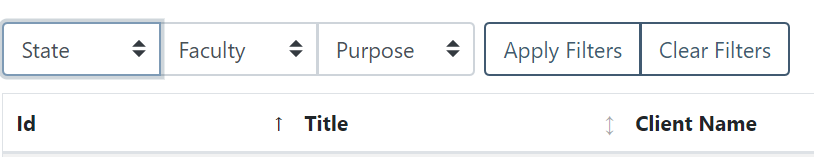
\includegraphics[width=3in]{Filter.png}\\
	\caption{State filter is selected}
	\label{fig:tobias}
\end{figure}
\begin{figure}[H]
	\centering
	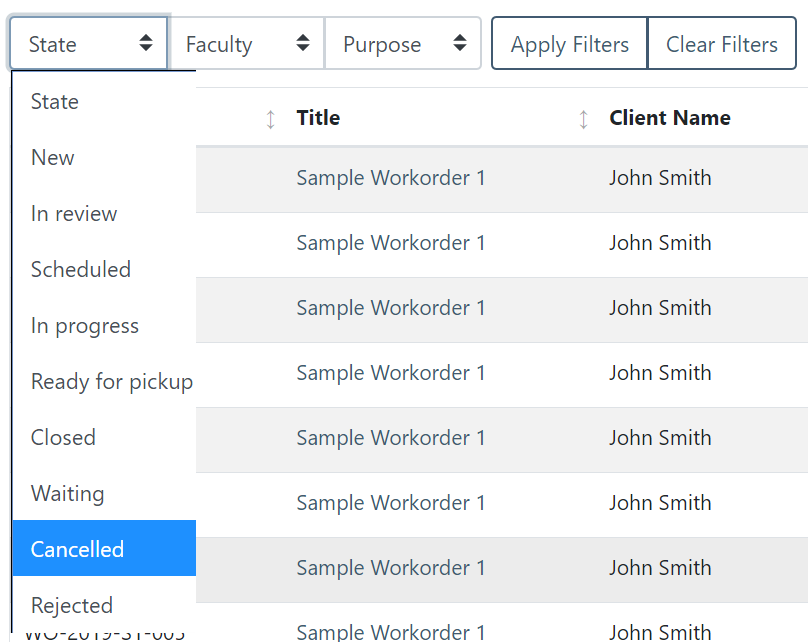
\includegraphics[width=3in]{filter-selected.png}\\
	\caption{Cancelled filter is being applied}
	\label{fig:tobias}
\end{figure}

Once the filter is chosen, the user can click on Apply Filters and the section will now only showcase the that are based on that filter.
\begin{figure}[H]
	\centering
	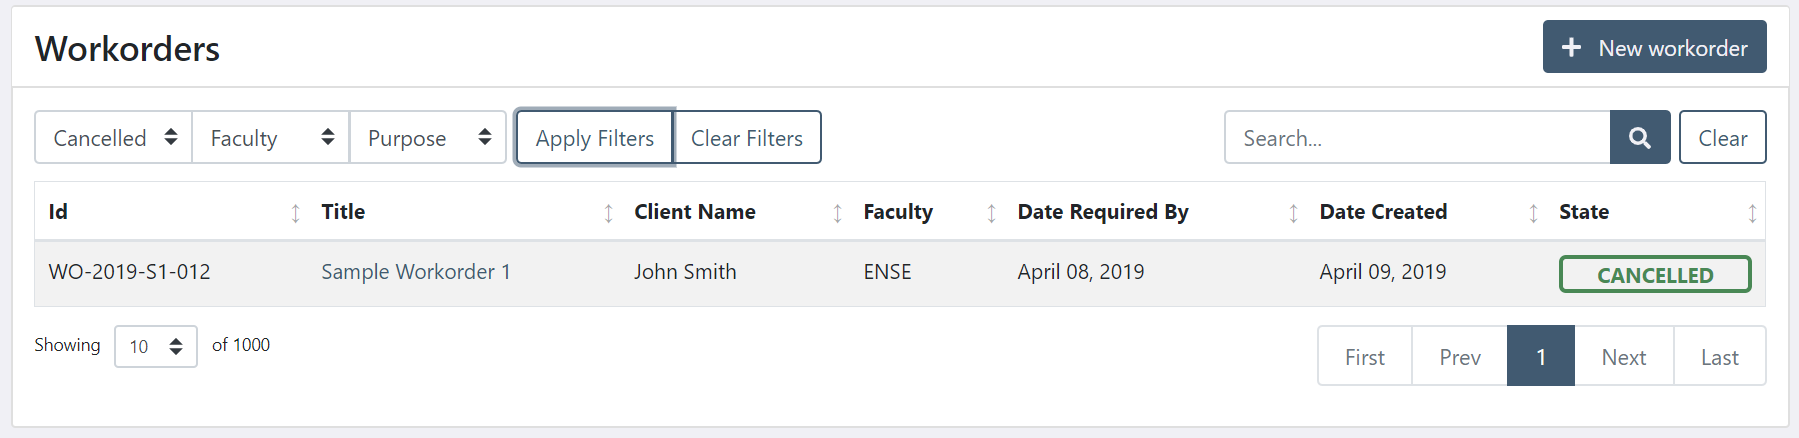
\includegraphics[width=5in]{cancelled.png}\\
	\caption{All cancelled workorders in table}
	\label{fig:tobias}
\end{figure}
To clear filters, the user can click on the Clear Filters button and the table will return to displaying all workorders. 
\newline
{\setlength{\parindent}{0cm}

To search for particular workorders, the user can type in what they are looking for in the search bar and click on the search button. The user can click on clear to remove all text from the search bar. 
\begin{figure}[H]
	\centering
	
\includegraphics[width=5in]{search.png}\\
	\caption{Searching}
	\label{fig:tobias}
\end{figure}

When the search button is clicked, then all workorders related to the specific text in the search bar is loaded into the table. 
\begin{figure}[H]
	\centering
	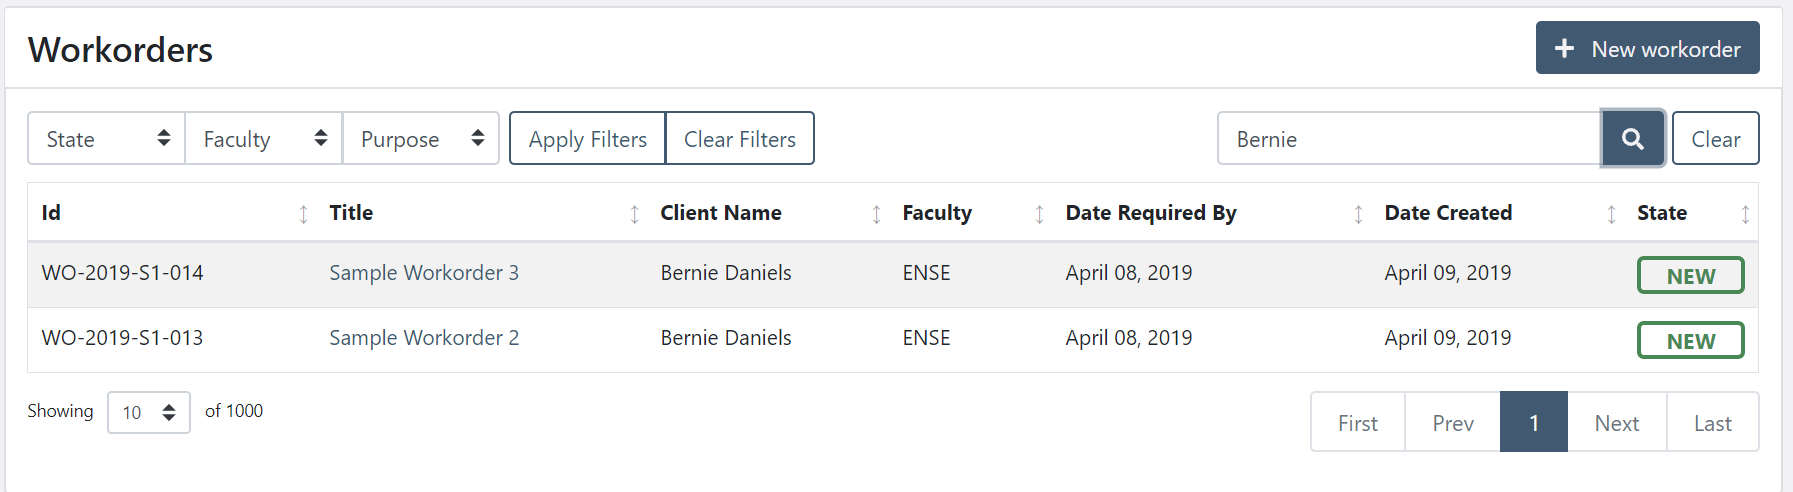
\includegraphics[width=5in]{searched-table.png}\\
	\caption{Table after searched}
	\label{fig:tobias}
\end{figure}

The table can also manipulated to showcase different amount of workorders on one page. 
\begin{figure}[H]
	\centering
	
\includegraphics[width=5in]{showing.png}\\
	\caption{Currently set to showing ten per page}
	\label{fig:tobias}
\end{figure}

The user can also go through the different pages to see more workorders in the table. 
\begin{figure}[H]
	\centering
	
\includegraphics[width=5in]{next.png}\\
	\caption{Number of pages in the workorders table}
	\label{fig:tobias}
\end{figure}

\newpage
\subsection{Workorder Details}
When a workorder is clicked on, a new page is loaded which contains all of the information regarding that workorder is associated with. Materials used in the workorder as well as any comments made about the workorder are located here. 
\begin{figure}[H]
	\centering
	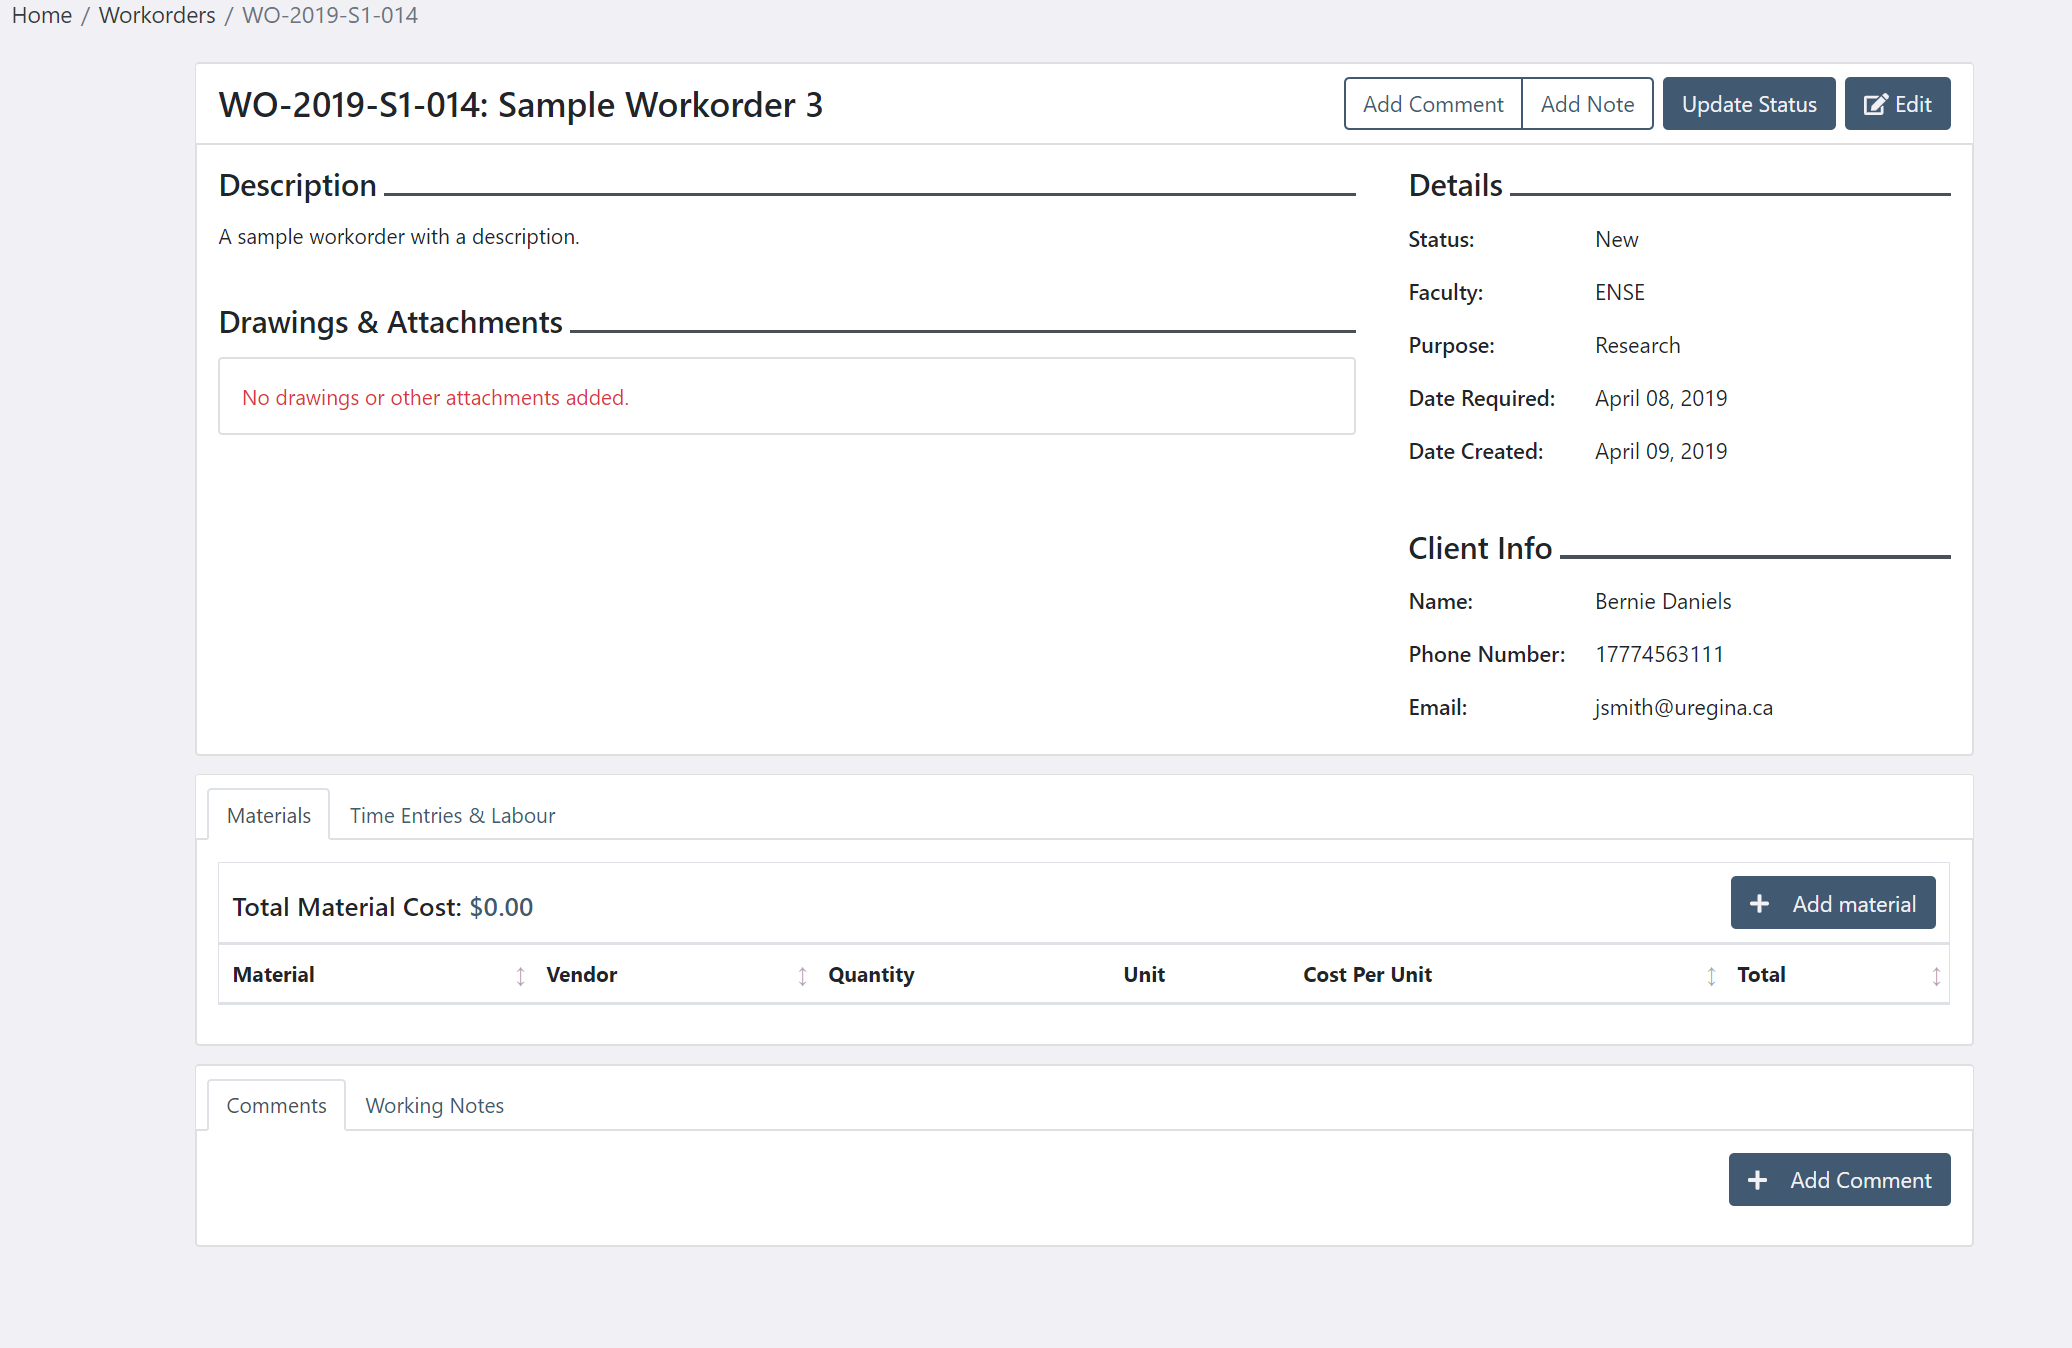
\includegraphics[width=5in]{details.png}\\
	\caption{Workorder details}
	\label{fig:tobias}
\end{figure}

To add a comment to the workorder, the user would click on the add comment button and submit their comment. 
\begin{figure}[H]
	\centering
	
\includegraphics[width=3in]{comment-button.png}\\
	\caption{Comment button selected}
	\label{fig:tobias}
\end{figure}

\begin{figure}[H]
	\centering
	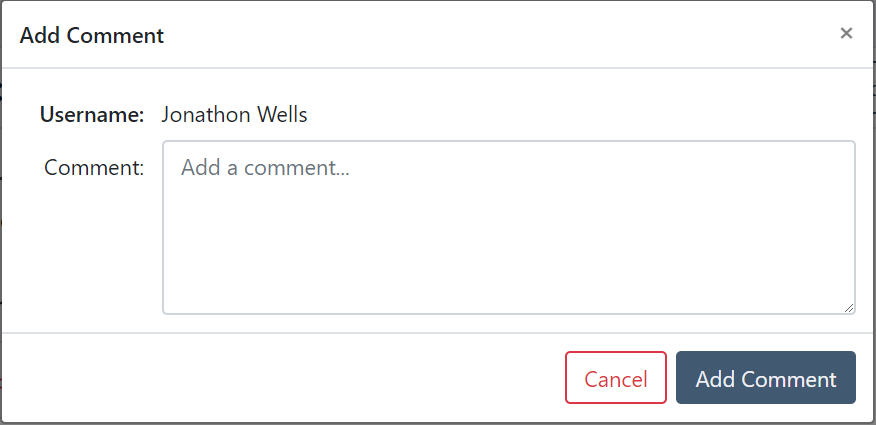
\includegraphics[width=5in]{add-comment.png}\\
	\caption{Comment submission form}
	\label{fig:tobias}
\end{figure}

\begin{figure}[H]
	\centering
	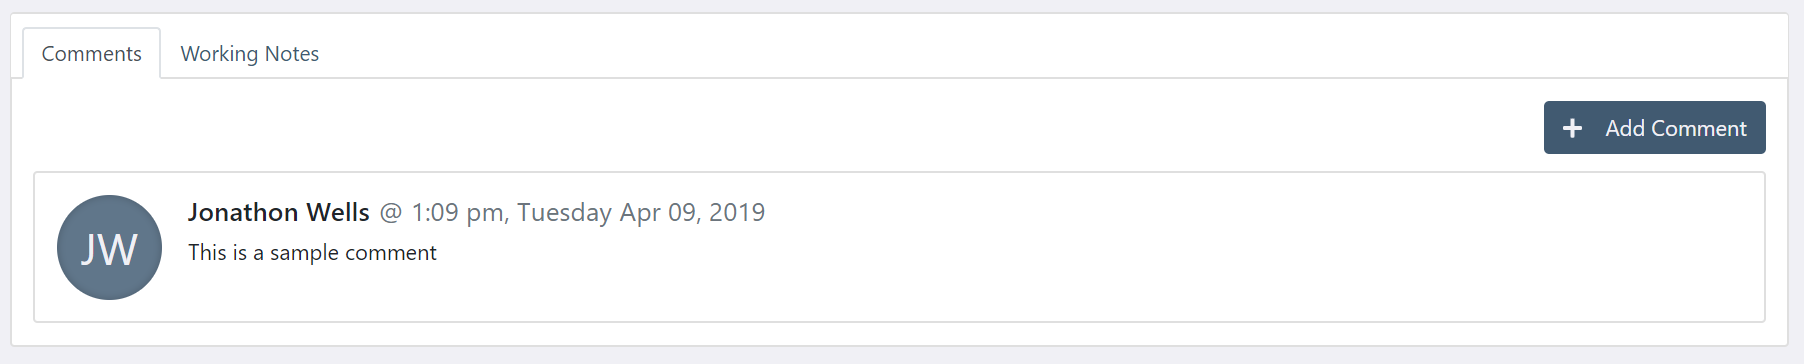
\includegraphics[width=5in]{comment.png}\\
	\caption{Comment created}
	\label{fig:tobias}
\end{figure}

Similarly, the user can chose to change the status of the particular workorder. 
\begin{figure}[H]
	\centering
	\includegraphics[width=3in]{Change-Status-button.png}\\
	\caption{Comment button selected}
	\label{fig:tobias}
\end{figure}

\begin{figure}[H]
	\centering
	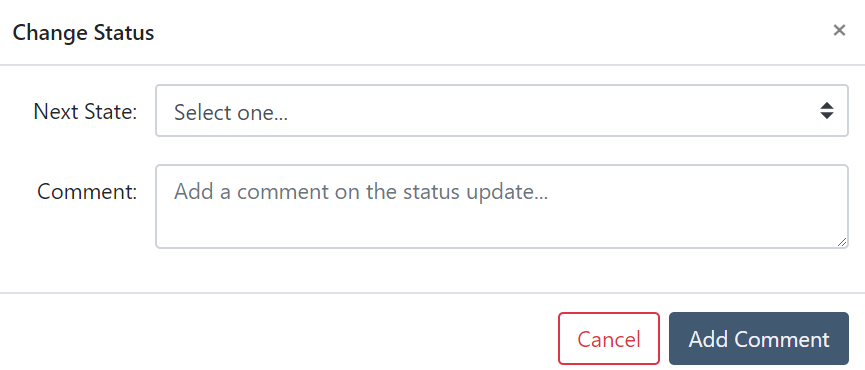
\includegraphics[width=5in]{add-change-status.png}\\
	\caption{Comment submission form}
	\label{fig:tobias}
\end{figure}

\newpage
\subsection{New Workorder}
After the user clicks on the new button, the new workorder section is loaded. 
\begin{figure}[H]
	\centering
	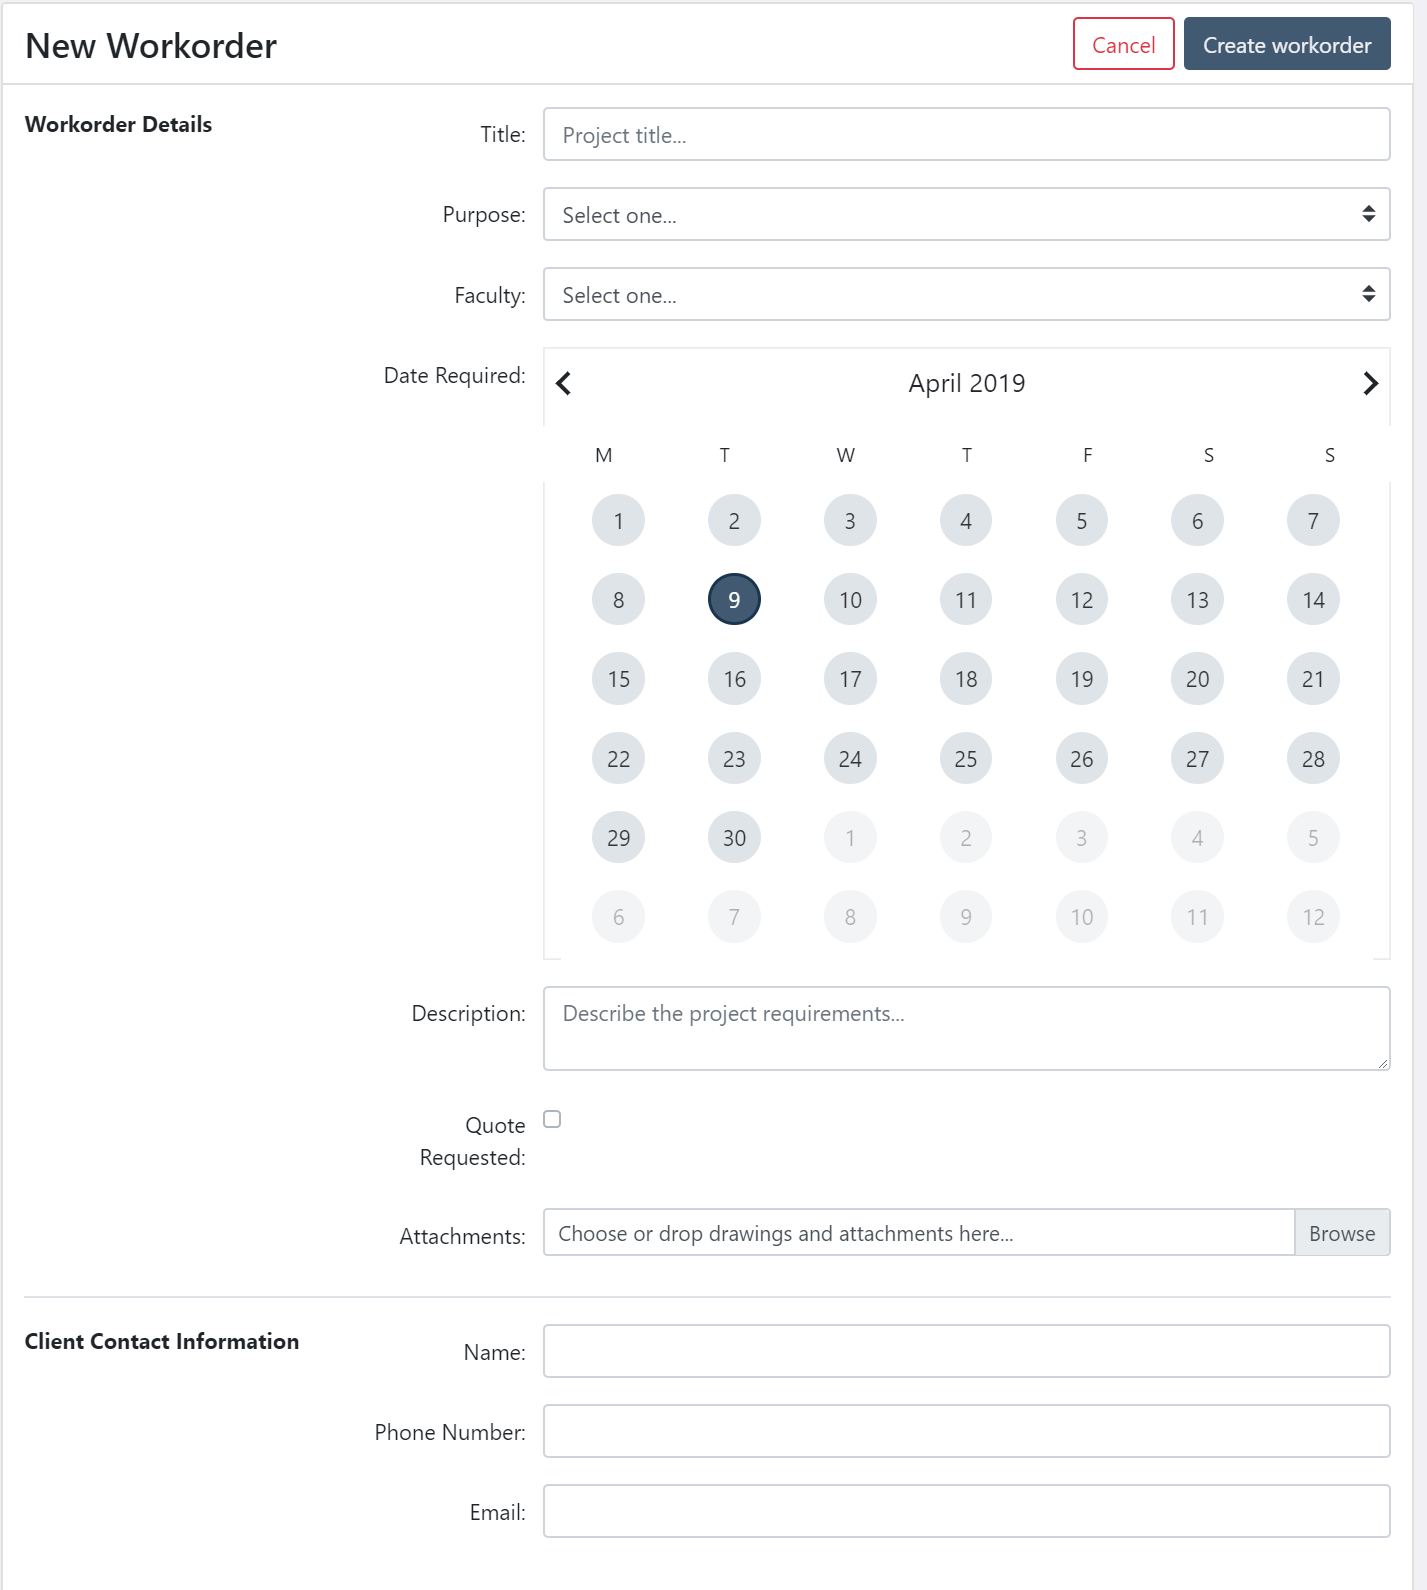
\includegraphics[width=5in]{new-workorder.png}\\
	\caption{Comment submission form}
	\label{fig:tobias}
\end{figure}

From here, the user adds the title of the workorder, select the faculty the client belongs to, the purpose of the workorder, date that project needs to be done by, and a description of the work. As well, the user can specify any attached attachments as well whether or not any estimates or quotes are needed. The user will then enter their user information so that the workshop manager can contact the workshop creator.

\newpage
\section{Materials}
This section specifies the materials section and how the user can then see all the materials inside the database.

\begin{figure}[H]
	\centering
	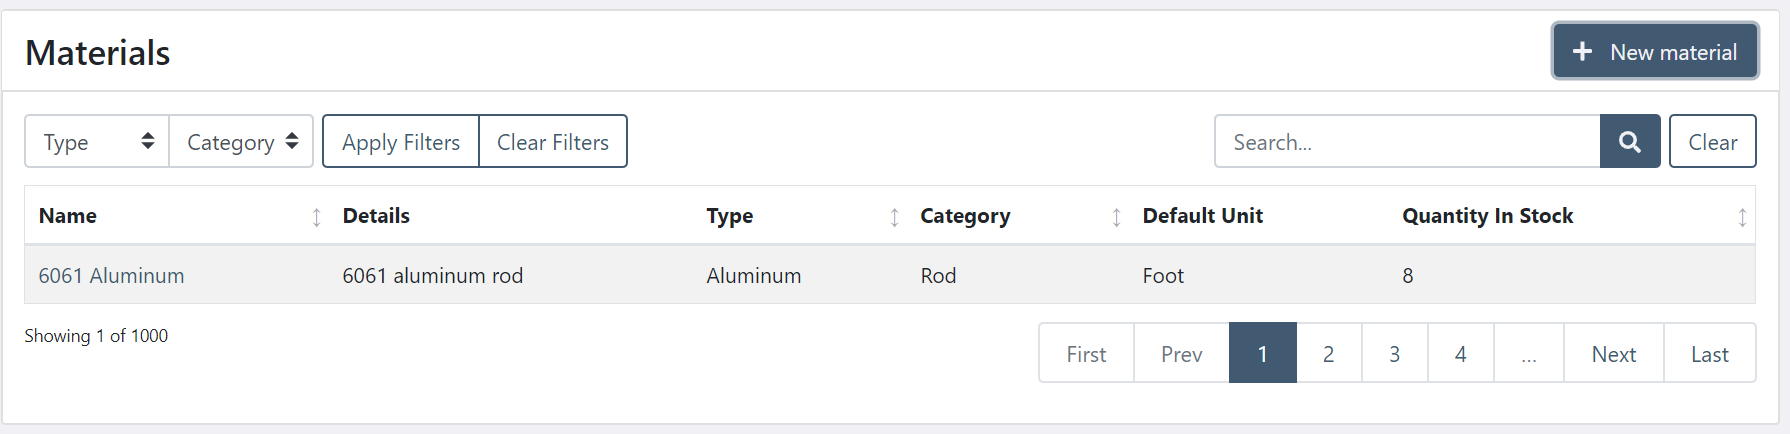
\includegraphics[width=5in]{material-table.png}\\
	\caption{Materials table}
	\label{fig:tobias}
\end{figure}

The table functions very similarly to the workorders table. It uses the same type of filtering and pagination, as well as the same type of search method. Materials can be clicked on and all data regarding the material is loaded. The default view for the calendar is by week, but there are options for month and day are available.

\section{Project Management}
The project management section showcases all the entries inside the database and is visualized in a calendar view. 

\begin{figure}[H]
	\centering
	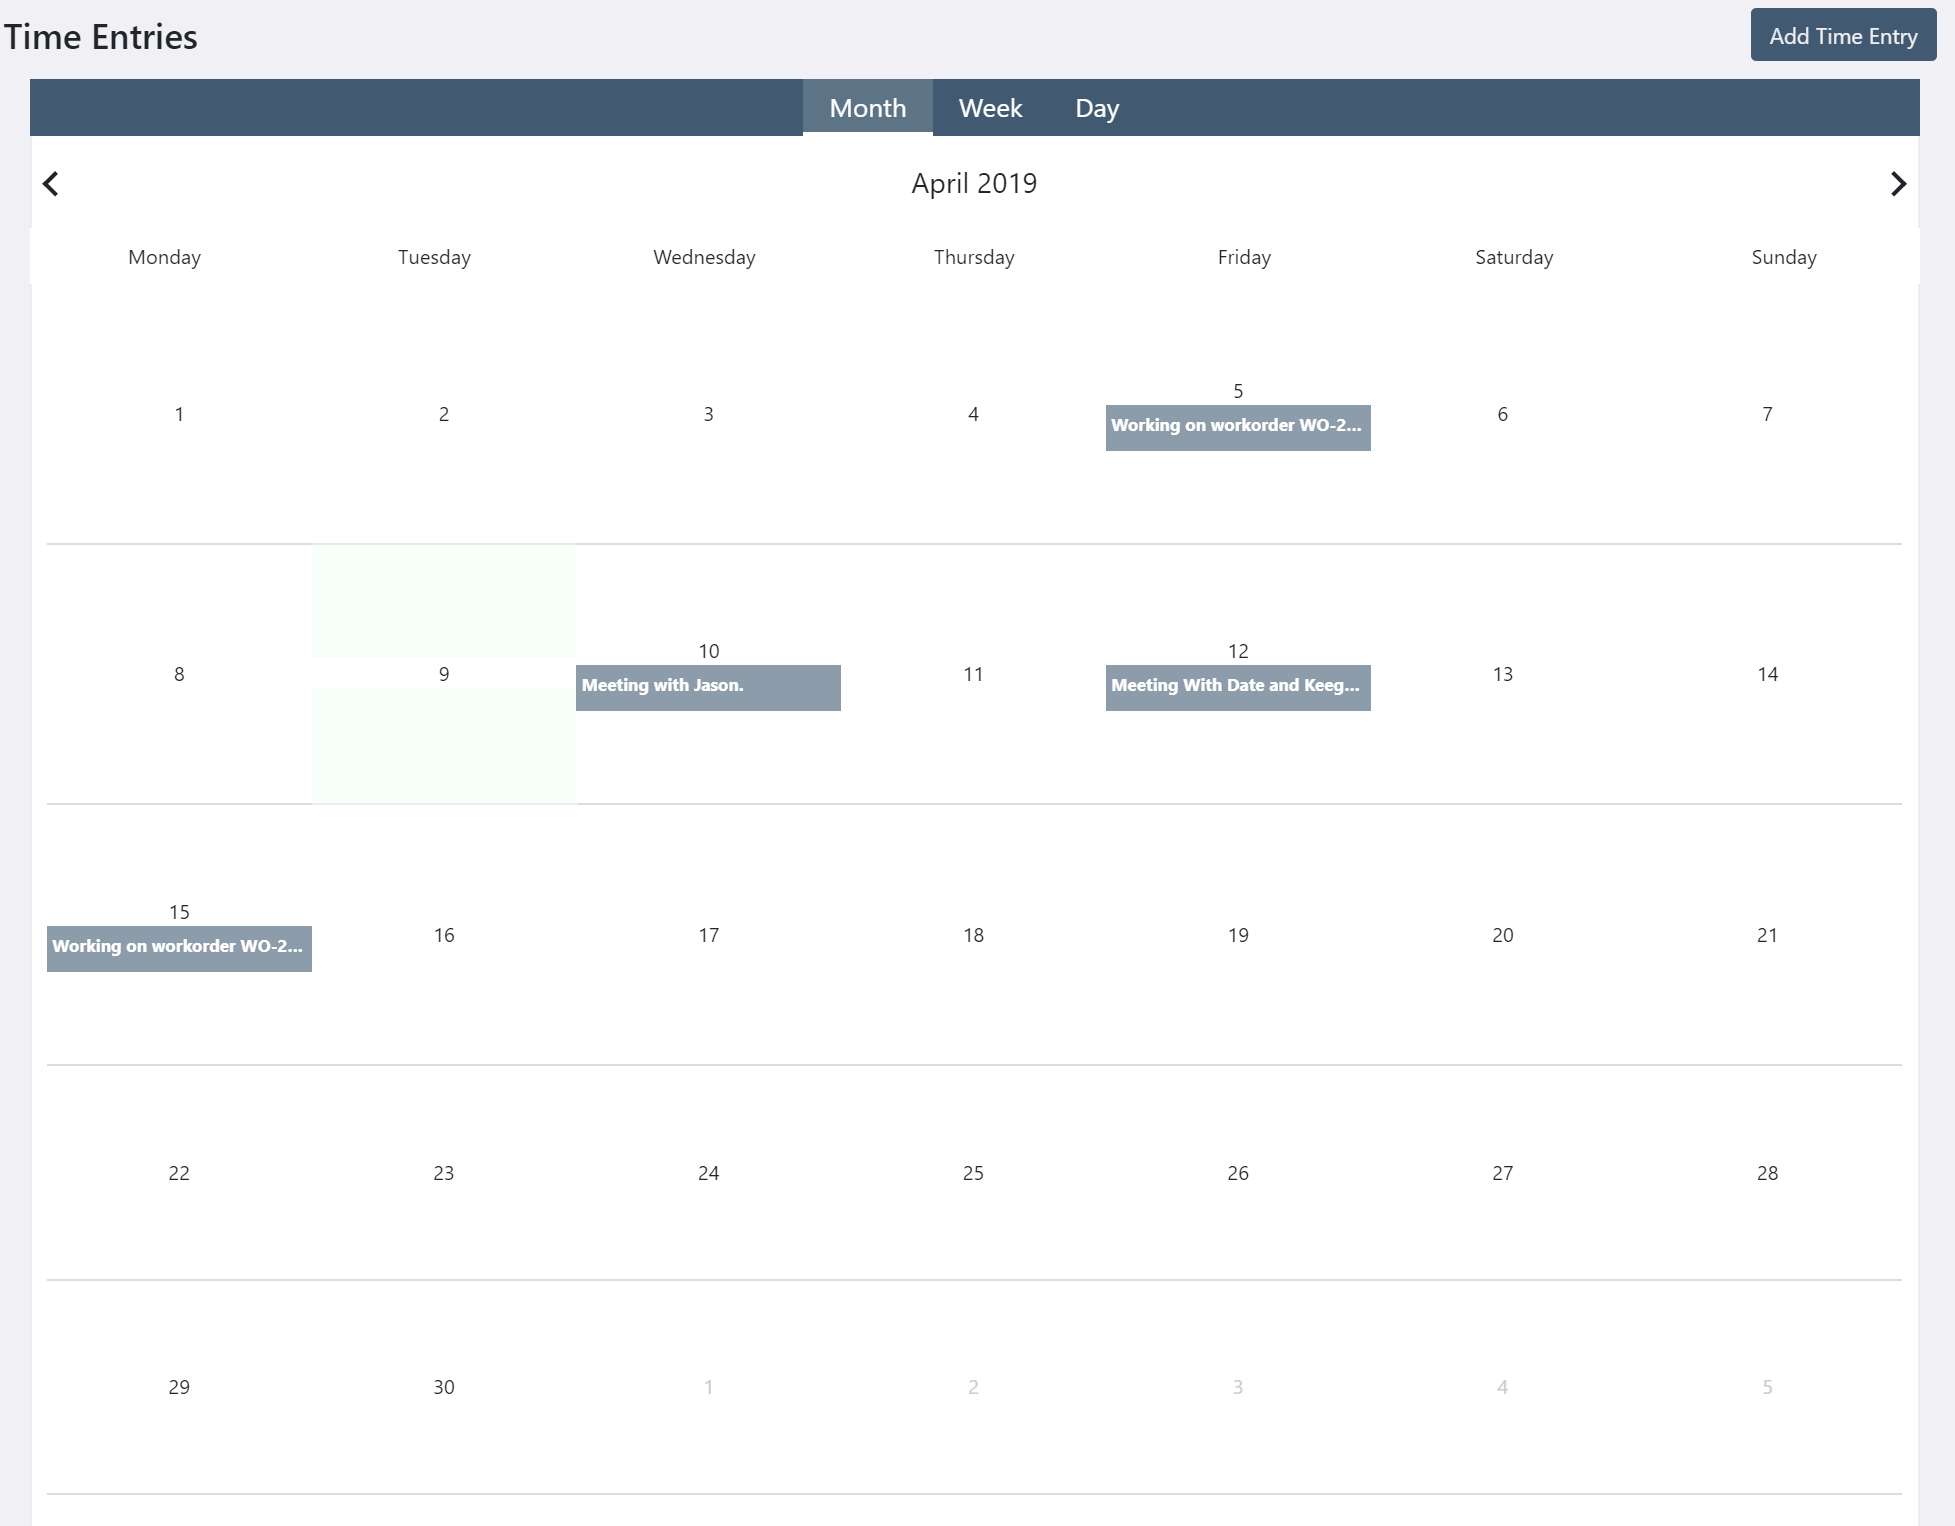
\includegraphics[width=5in]{calendar-month.png}\\
	\caption{Calendar by month}
	\label{fig:tobias}
\end{figure}

\begin{figure}[H]
	\centering
	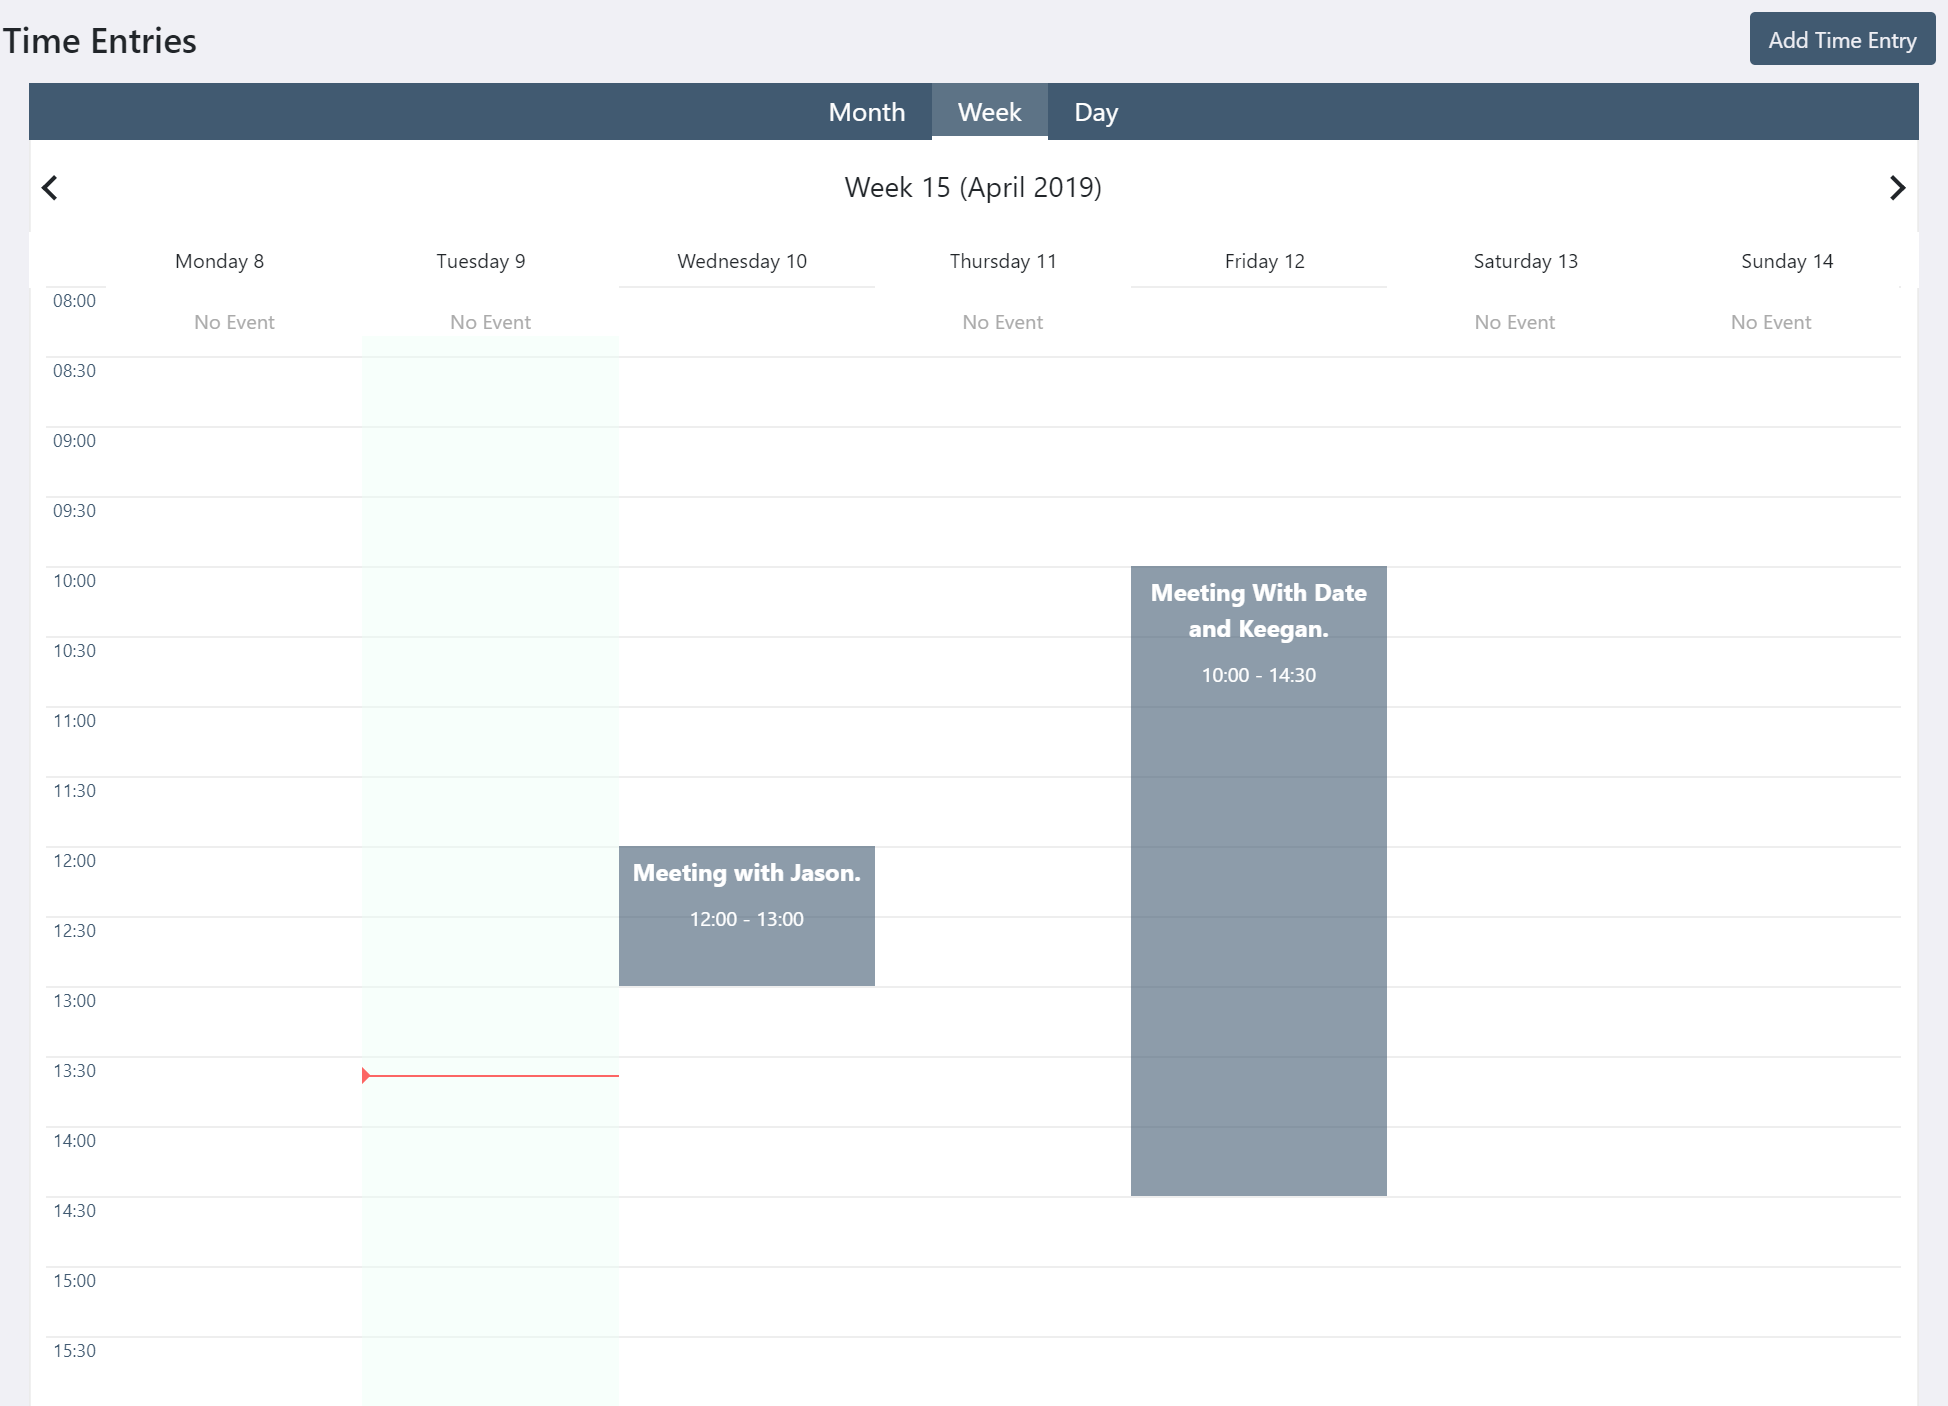
\includegraphics[width=5in]{calendar-week.png}\\
	\caption{Calendar by week}
	\label{fig:tobias}
\end{figure}

\begin{figure}[H]
	\centering
	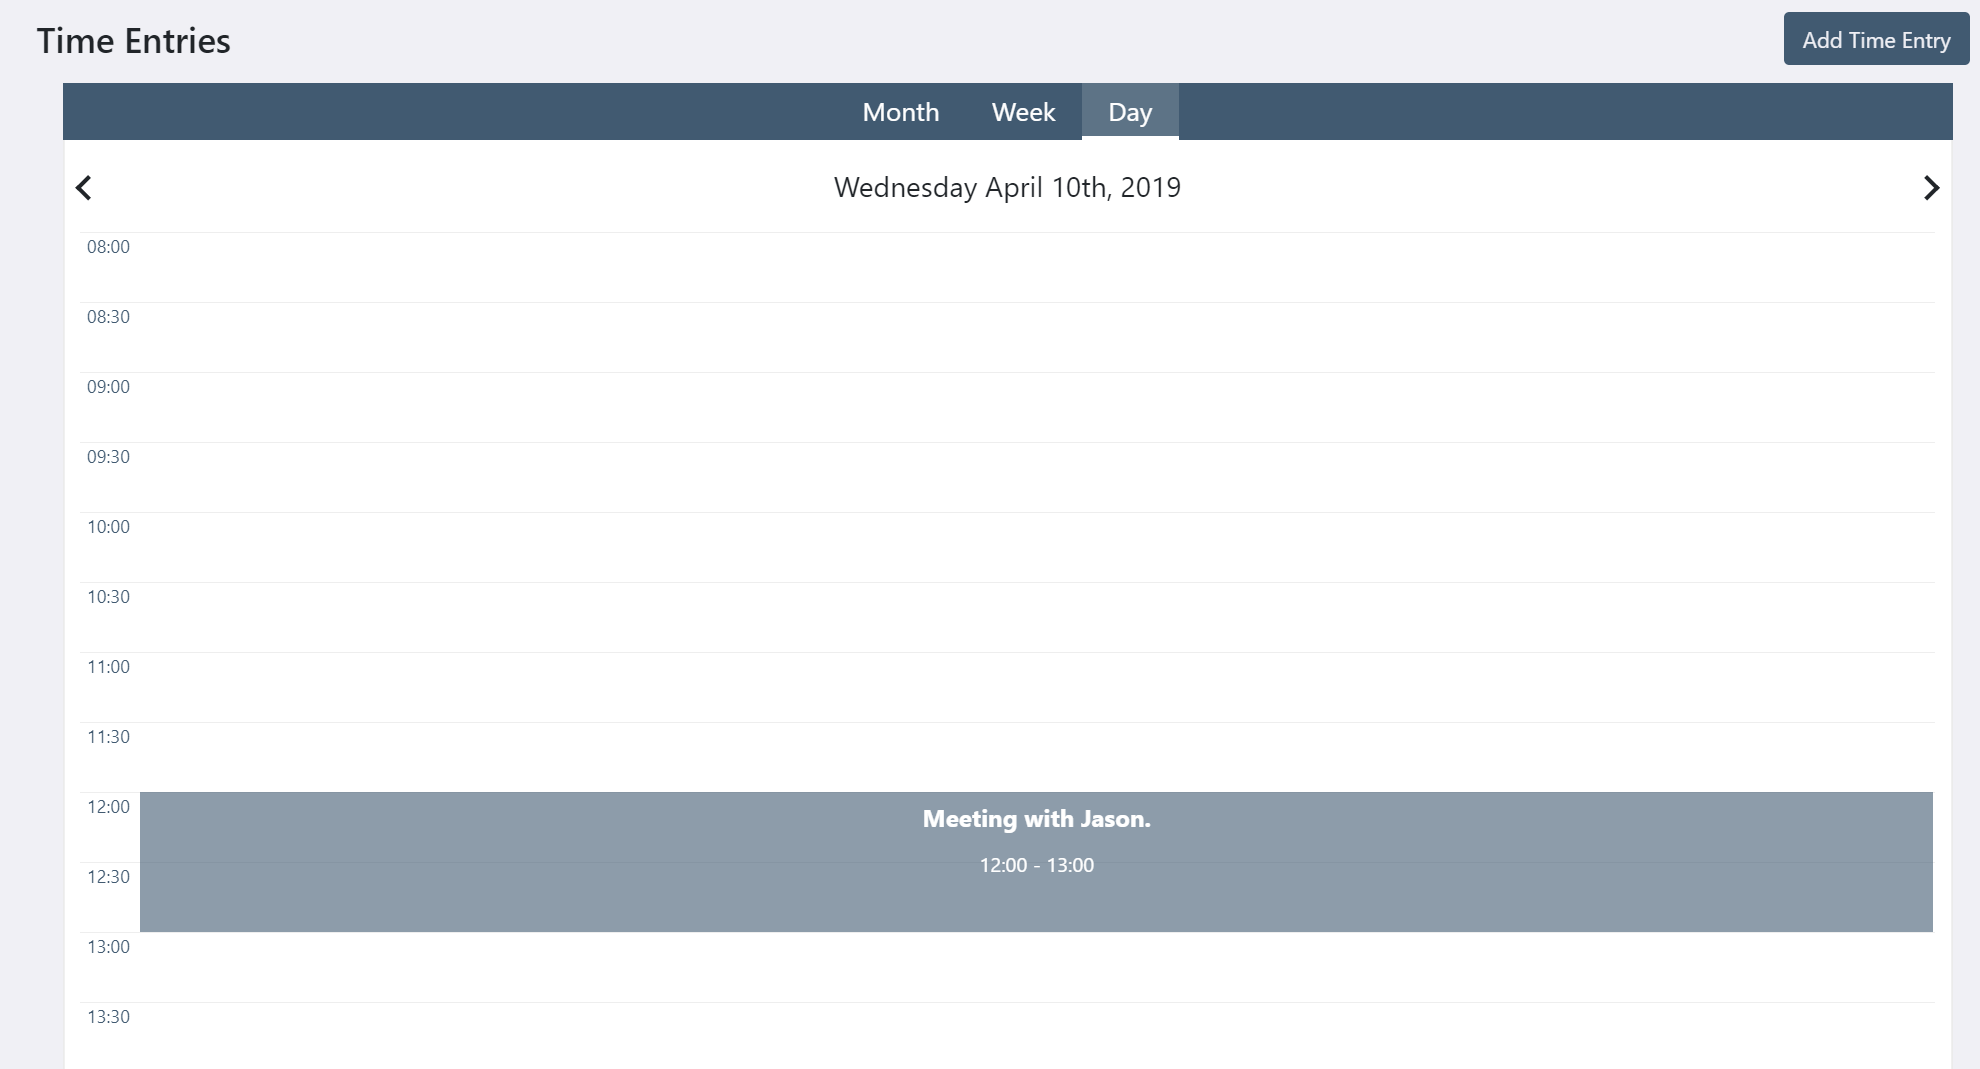
\includegraphics[width=5in]{calendar-day.png}\\
	\caption{Calendar by day}
	\label{fig:tobias}
\end{figure}

\newpage
\section{Project Management Quick Access}
On the right hand side menu, the user can access the project management quick access menu, which showcases any notifications for the user as well as a quick view of the day. This menu is accessible from any page in the application.
\newline
{\setlength{\parindent}{0cm}

The top feature is the notifications tab, where any new entries such as new comments and new workorders can be seen.
\begin{figure}[H]
	\centering
	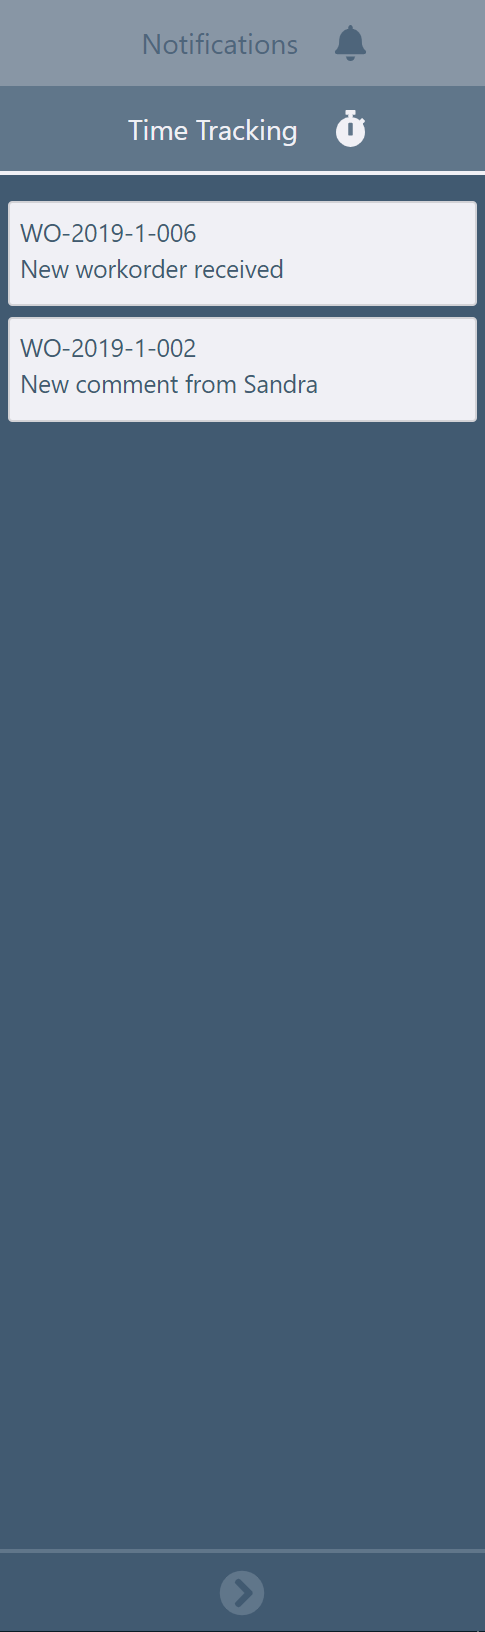
\includegraphics[width=2in]{pmqa-notifications.png}\\
	\caption{the notifications centre in the PMQA}
	\label{fig:tobias}
\end{figure}

The feature below is time tracking, where all events in the current day can be viewed. There is also an indicator showcasing the current time of the day. 
\begin{figure}[H]
	\centering
	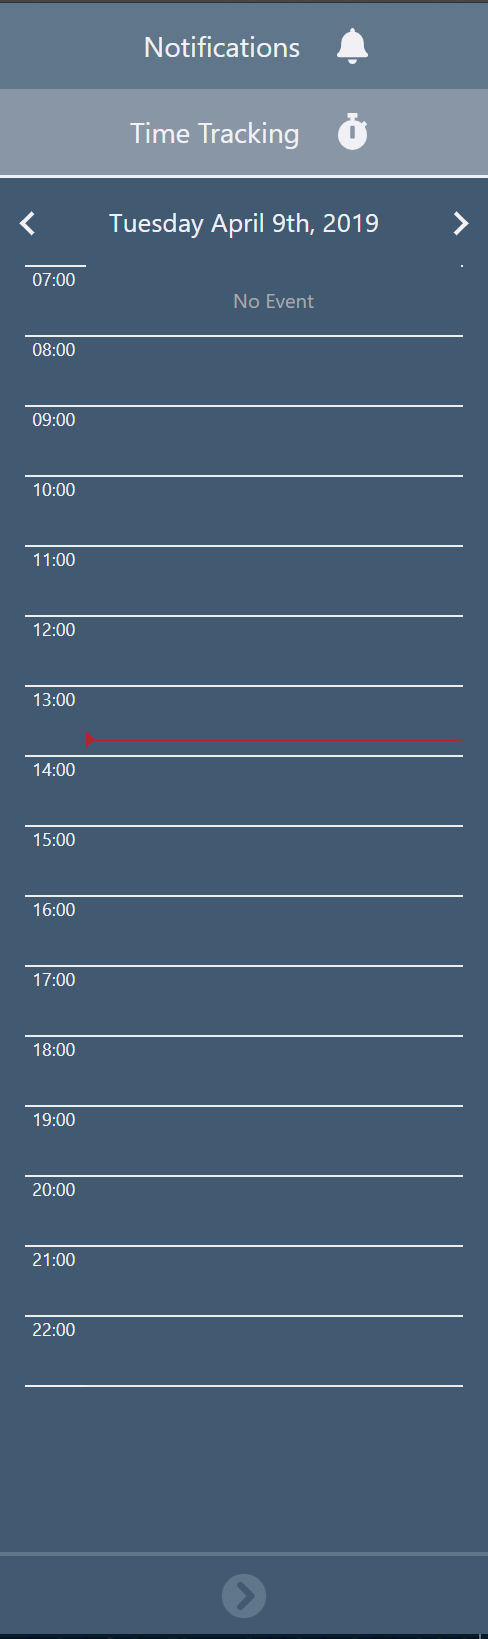
\includegraphics[width=2in]{pmqa-calendar.png}\\
	\caption{the calendar in the PMQA}
	\label{fig:tobias}
\end{figure}

Just like the side menu on the left, the bottom arrow can condense the PMQA menu.
\begin{figure}[H]
	\centering
	
\includegraphics[width=0.3in]{pmqa-condensed.png}\\
	\caption{PMQA condensed}
	\label{fig:tobias}
\end{figure}

\end{document}


